\section{Koopman Operator Theory}
A continuous time dynamical system can at its simplist be considered in the following form:

\begin{equation}
    \diff{\mathbf{x}(t)}{t} = \mathbf{f}\left(\mathbf{x}(t), t; \boldsymbol{\beta}\right)
\end{equation}

A discrete time system can analogously be considered in the following form:

\begin{equation}
    \mathbf{x}_{k + 1} = \mathbf{F}(\mathbf{x}_k, t; \mathbb{\beta})
    \label{eq:discrete_dynamical_system}
\end{equation}

Koopman operator theory states that it is possible to represent a nonlinear dynamical system in terms of an
infinite-dimensioned linear operator acting on a Hilbert space of measurement functions of the state of the system
\parencite{bruntonDatadrivenScienceEngineering2019}. This was demonstrated by
\citeauthor{koopmanHamiltonianSystemsTransformation1931} in \citeyear{koopmanHamiltonianSystemsTransformation1931}. This
operator is linear, making analysis of the system much easier. It is however infinite, so must be truncated for real
applications. 

\subsection{Mathematical Formulation}
The Koopman operator is a linear operator that acts on a measurement function as follows:
\begin{equation}
    \mathcal{K} g = g(\mathbf{F})
\end{equation}
For a discrete system as described in \eqref{eq:discrete_dynamical_system}, this formulation becomes the following:

\begin{align}
    \mathcal{K}g(\mathbf{x}_k) = g(\mathbf{F}(\mathbf{x}_k)) \\
    \mathcal{K} g(\mathbf{x}_k) = g(\mathbf{x}_{k + 1})
\end{align}

This means the Koopman Operator is a linear operator that advances the observation of a state forward in time. This is
true for any observable function \( g\) and any state \( \mathbf{x}_k \). \Cref{fig:koopman_visualisation} visualises
the transformation performed by the Koopman operator and the measurement functions.

\begin{figure}[H]
    \centering
    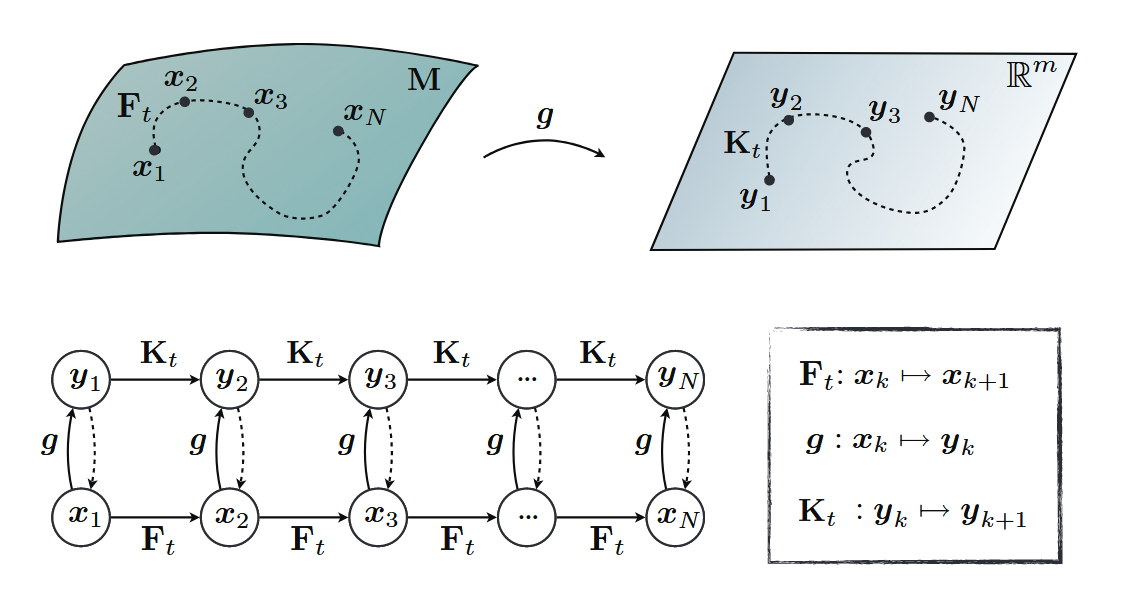
\includegraphics[width=0.75\linewidth]{report/images/literature_study/bruntonDataDrivenDynamicalSystems2019.png}
    \caption{Schematic illustrating the Koopman operator for nonlinear dynamical systems. The dashed lines from yk → xk
    indicate that we would like to be able to recover the original state.
    \parencite{bruntonDataDrivenDynamicalSystems2019}}
    \label{fig:koopman_visualisation}
\end{figure}

The operator is however infinite in dimension. This provides a significant challange for computing. Instead of capturing
the development of all the measurement functions, one can identify key measurement functions that evolve linearly over time.
\parencite{bruntonDatadrivenScienceEngineering2019}. This can be done by determining the eigenfunctions of the koopman
operator \( (\varphi(\mathbf{x}_k)) \). 

\begin{equation}
    \varphi(\mathbf{x}_{k + 1}) = \mathcal{K}\varphi(\mathbf{x}_k) = \lambda \varphi(\mathbf{x}_k)
\end{equation}

These eigenfunctions allow one to globally model nonlinear dynamics with a linear representation. A set of Koopman
eigenfunctions can be used to generate more eigenfunctions. The product of two eigenfunctions is also an eigenfunction.

\begin{align}
    \mathcal{K}(\varphi_1(\mathbf{x})\varphi_2(\mathbf{x})) &= \varphi_1(\mathbf{F}(\mathbf{x}))\varphi_2(\mathbf{F}(\mathbf{x})) \\
    &=\,\lambda_1\lambda_2\varphi_1(\mathbf{x})\varphi_2(\mathbf{x})
\end{align}

This means there may be a finite set of eigenfunctions that can be used to construct all infinite eigenfunction needed
to fully represent the nonlinear system. 

\subsubsection{Finite dimensional models}

As the eigenfunctions form a basis for the measurement space, each measurement function can be formualated as an
infinite weighted sum of eigenfunctions.

\begin{equation}
    g_i(\mathbf{x}) = \sum_{j = 1}^{\infty} v_{ij}\varphi_j(\mathbf{x})
    \label{eq:koopman_measurement_spec_decomp}
\end{equation}

If we consider a measurement vector \(\mathbf{g}(\mathbf{x}) = [g_1(\mathbf{x}), \dots, g_p(\mathbf{x})]^T \),
\eqref{eq:koopman_measurement_spec_decomp} can be formulated in vector form:

\begin{equation}
    \mathbf{g}(\mathbf{x}) = \begin{bmatrix}
        g_1(\mathbf{x}) \\
        g_2(\mathbf{x}) \\
        \vdots         \\
        g_p(\mathbf{x})
    \end{bmatrix}
    = \sum_{j = 1}^{\infty} \varphi_j(\mathbf{x}) \mathbf{v}_j
\end{equation}
Where \(\mathbf{v}_j\) is the $\mathit{j}$-th Koopman mode associated with $\varphi_j$. For practical applications, this
sum is truncated to make an approximation of the measurement space. The challenge of using the Koopman operator has now
shifted to selecting the best finite set of eigenfunctions to capture the systems dynamics.

\subsection{Data-driven Koopman analysis}
Analytically Determining the Koopman eigenfunctions and their weights for a complex non-linear dynamical system is not
practically feasible. As such data-driven techniques are the method of choice for real world systems. Several techniques
will be discussed in this section, starting with dynamic mode decomposition (DMD). Augmented and extended DMD will then
be covered as will as integration with SINDy approaches. Finally a neural network approach will be covered.
\subsubsection{Dynamic mode decomposition}
DMD is a data driven technique used to identify modes that represent spatial patterns that evolve linearly in time. DMD
approximates the Koopman operator while restricted to a set of direct measurements of the state. It is based purely on
data, and requires no prior knowledge of the system's governing equations. Its simple and efficient numerical
implementation has made it popular in recent years \parencite{bruntonDataDrivenDynamicalSystems2019}. 

The governing principle is as follows: Snapshots of the dynamical system are arranged into two data matrices. These
matrices are then used to solve for a linear operator that maps one data matrix onto the other. 

\begin{equation}
    \label{eq:dmd_X_matrices}
    \begin{split}
    \mathbf{X} &= \left[\mathbf{x}(t_1), \mathbf{x}(t_2),\dots,\mathbf{x}(t_m) \right] \\
    \mathbf{X'} &= \left[\mathbf{x}(t'_1), \mathbf{x}(t'_2),\dots,\mathbf{x}(t'_m) \right]
\end{split}
\end{equation}

\begin{equation}
    \mathbf{X'} \approx \mathbf{AX}
\end{equation}
DMD provides a method for obtaining $\mathbf{A}$ efficiently using a singular value decompostion of $\mathbf{X}$.

This method can be extended by using a library of nonlinear measurement functions and fitting a linear operator to the
augmented state.

\begin{equation}
    \mathbf{y} = \Theta^T(\mathbf{x}) = \begin{bmatrix}
        \theta_1(\mathbf{x})\\
        \theta_2(\mathbf{x})\\
        \vdots\\
        \theta_p(\mathbf{x})
    \end{bmatrix}
\end{equation}

Then two augmented data matrices are constructed, analogously to \eqref{eq:dmd_X_matrices}. These can then be solved to
obtain a linear operator. If $\Theta$ fully spans a Koopman invarient subspace, the extended DMD operator converges to
the Koopman operator in the limit of $m$. However, if $\Theta$ contains the wrong functions, the model will overfit or
give incorrect modal responses. Correctly determining the functions that should be contained in $\Theta$ is thus
essential.

\subsubsection{Hankel-DMD}
A variant of DMD is Hankel-DMD. Instead of just considering the transformation of the current state, the Hankel-DMD
approach includes time-delayed measurements \parencite{bruntonDataDrivenDynamicalSystems2019}. This allows the Koopman transformation to include longer term memory
effects. 

\TODO{Sparse identification of koopman eigenfunctions

motivation for identifying eigenfunctions rather than entire matrix:

- Identifying regression models based on nonlinear measurements will
generally result in closure issues \parencite{luschDeepLearningUniversal2018}\\
- Resulting models are often high dimension, can become uninterpretable

- In practice obtaining eigenfunctions is difficult
}

\subsubsection{Neural networks for Koopman theory}
Even for relatively simple dynamical systems, the Koopman eigenfunctions can be arbitrarily complex
\parencite{bruntonDataDrivenDynamicalSystems2019}. Creating a suitable library for use with eDMD can be challenging.
Deep learning could provide an alternative approach \textcite{luschDeepLearningUniversal2018}

The goal of determining an invertable function \(\varphi\) and Koopman operator \(\mathcal{K}\) such that \( y_{k} =
\varphi(x_k) \) and \( y_{k + 1} = \mathcal{K}y_k \). This problem fits well with a deep auto-encoder based approach. An
additional constraint added is that the dynamics of the latent variables must linarly represent the dynamics of the
system. This forces the encoder to act as Koopman eigenfunctions. 

\begin{figure}[H]
    \centering
    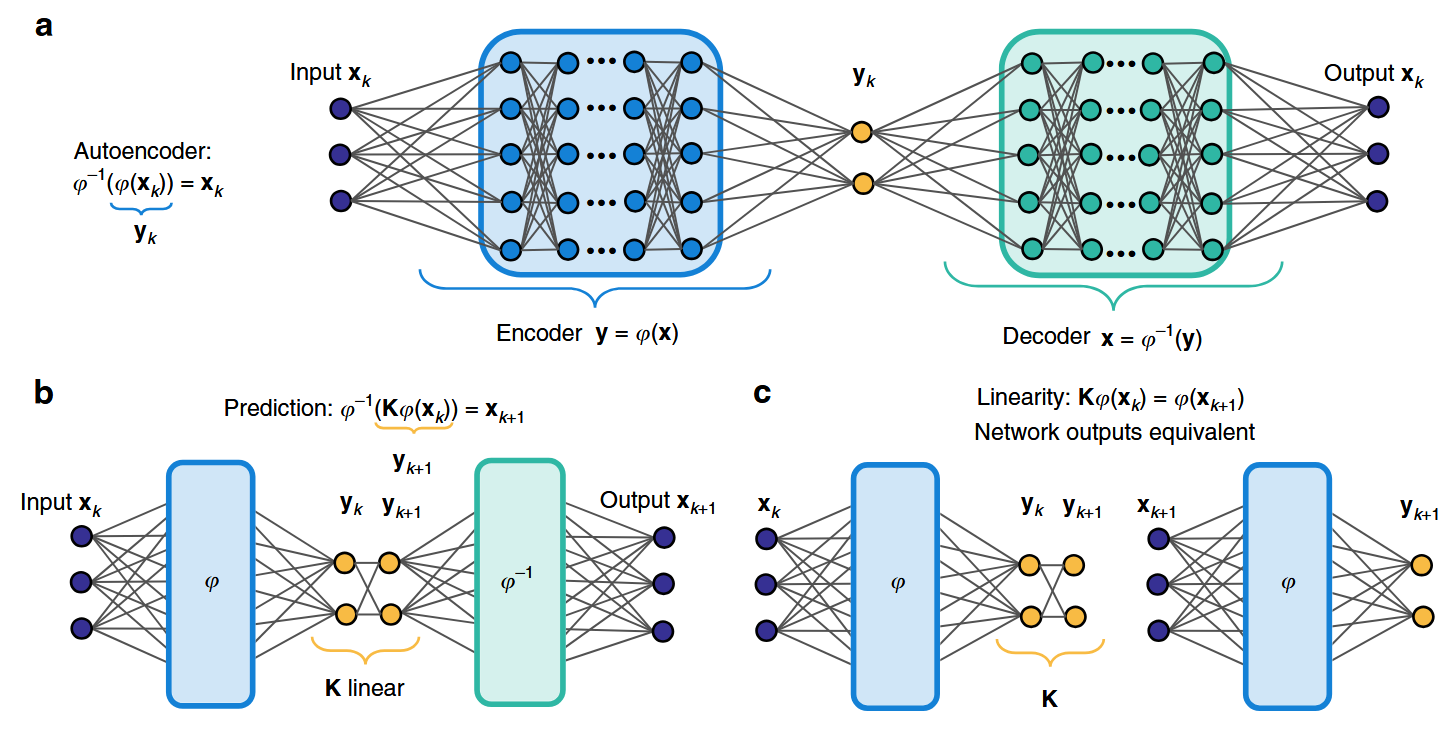
\includegraphics[width=\linewidth]{report/images/literature_study/luschDeepLearningUniversal2018.png}
    \caption{Deep neural network architecture used to identify Koopman eigenfunctions φ(x). The network is based on a
    deep auto-encoder (a), which identifies intrinsic coordinates y = φ(x). Additional loss functions are included to
    enforce linear dynamics in the auto-encoder variables (b,c) \parencite{luschDeepLearningUniversal2018}}
    \label{fig:lusch_koopman_AE_architecture}
\end{figure}

In the case where the system has continuous eigenvalues, the neural net representing \(\mathcal{K}\) can be parametrized
for the eigenvalue of the system. This can be obtained with another neural net on the latent variables.
\textcite{luschDeepLearningUniversal2018} indicate this approach still works on systems that have discrete Koopman
eigenvalues, meaning no prior knowledge is needed on the nature of the Koopman eigenvalues. 

This approach is not without its challenges. While there is no more need to select a basis for the eDMD method, one now
has to decide on the number of latent nodes needed, as well as other hyperparameters. This approach also has a larger
upfront computational cost to train the system as well as needing a large amount of data.

\subsection{Koopman theory for stochastic systems}
The above sections discuss the Koopman operator for deterministic systems. If a stochastic dynamical system is to be
considered however, the formulation can be adjusted. This is given by \textcite{crnjaric-zicKoopmanOperatorSpectrum2020}
in the following form: 

\begin{equation}
    \mathcal{K}g(\mathbf{x}) = \mathbb{E}[g(\mathbf{F}(\mathbf{x}))]
\end{equation}

\todo{check equation}

The eigenvalue formulation can then analogously be formulated:

\begin{equation}
    \mathcal{K}\varphi(\mathbf{x}) = \lambda^S(t)\varphi(\mathbf{x})
\end{equation}

where $\varphi$ are the eigenfunctions of the stochastic Koopman Operator and $\lambda^S(t)$ are the stochastic Koopman
eigenvalues. The stochastic Koopman operator tracks how the expected state of the stochastic dynamical system develops
in measurement space. It does not however track the variance of the the state.

\textcite{crnjaric-zicKoopmanOperatorSpectrum2020} discusses two approactes for determining the stochastic Koopman
operator. Both are based on the DMD approach, applied to the expected value of the measured state rather than on
deterministic tracjectories. The first is a modification of the regular DMD approach, while the second modifies the
Hankel-DMD approach. These methods do not inherintly consider the probability distrubution of the resulting
trajectories however.


\todo{Update text on VAMP}
Both VAMP \parencite{mardtVAMPnetsDeepLearning2018} and \textcite{zhaoDatadrivenProbabilityDensity2023} aim to approximate the Koopman operator using time-lagged covariance matrices derived from observed data. VAMP employs a variational principle to optimize the approximation within a chosen feature space, formulating the problem through the maximization of a score function based on covariance and cross-covariance matrices. \textcite{zhaoDatadrivenProbabilityDensity2023} adopt a conceptually similar framework but introduce alternative notation and implementation details, while retaining the core idea of leveraging covariance structures to estimate the operator. In essence, both methods share the same mathematical foundation, differing primarily in presentation and specific optimization strategies.

https://scholar.google.com/scholar?q=related:cdgg75wUJSYJ:scholar.google.com/&scioq=vampnet&hl=en&as_sdt=0,5&inst=6173373803492361994



